\documentclass[11.5pt]{sig-alternate} % sets document style to sig-alternate
% packages
% typesetting
%\usepackage{dirtytalk} % typset quotations easier (\say{stuff})
\usepackage{hanging} % hanging paragraphs
\usepackage[defaultlines=3,all]{nowidow} % avoid widows
\usepackage[pdfpagelabels=false]{hyperref} % produce hypertext links, includes backref and nameref
\usepackage{xurl} % defines url linebreaks, loads url package
\usepackage{microtype}
\usepackage{textgreek}
%\usepackage{textcomp}
%\newcommand{\texttildemid}{\raisebox{0.4ex}{\texttildelow}}
% layout
\usepackage{enumitem} % control layout of itemize, enumerate, description
\usepackage{fancyhdr} % control page headers and footers
\usepackage{float} % improved interface for floating objects
%\usepackage{multicol} % intermix single and multiple column pages
% language
\usepackage[utf8]{inputenc} % accept different input encodings
\usepackage[english]{babel} % multilanguage support
% misc
\usepackage{graphicx} % builds upon graphics package, \includegraphics
%\usepackage{lastpage} % reference number of pages
%\usepackage{comment} % exclude portions of text (?)
\usepackage{xcolor} % color extensions
\usepackage[backend=biber, style=apa]{biblatex} % sophisticated bibliographies % necessary for HTML to display author info and date on abstract page
\usepackage{csquotes} % advanced quotations, makes biblatex happy
\usepackage{authblk} % support for footnote style author/affiliation
% tables and figures
\usepackage{tabularray}
%\usepackage{array} % extend array and tabular environments
\usepackage{caption} % customize captions in figures and tables (rotating captions, sideways captions, etc)
%\usepackage{cuted} % allow mixing of \onecolumn and \twocolumn on same page
\usepackage{multirow} % create tabular cells spanning multiple rows
%\usepackage{subfigure} % deprecated, support for manipulation of small figures
%\usepackage{tabularx} % extension of tabular with column designator "x", creates paragraph-like column whose width automatically expands
%\usepackage{wrapfig} % allows figures or tables to have text wrapped around them
%\usepackage{booktabs} % better rules
% dummy text
%\usepackage{blindtext} % blind text dummy text
%\usepackage{kantlipsum} % Kant style dummy text
\usepackage{lipsum} %lorem ipsum dummy text
% other helpful packages may be booktabs, longtable, longtabu, microtype

\pagestyle{fancy} % sets pagestyle to fancy for fancy headers and footers

% header and footer
% modern way to set header image
\renewcommand{\headrulewidth}{0pt} % defines thickness of line under header
\renewcommand{\footrulewidth}{0pt} % defines thickness of line above header
\setlength\headheight{80.0pt} % sets height between top margin and header image, effectively moves page contents down
\addtolength{\textheight}{-80.0pt} % seems to affect the lower height. maybe only works properly if footer numbers enabled?
\fancyhf{}
\fancyhead[CE, CO]{
\includegraphics[width=\textwidth]{headerImage.png}}
% footer
%\fancyfoot[LE,LO]{Article Title Here \\ DOI: }% left footer article title and doi
%\fancyfoot[CE,CO]{{}} % center footer empty
%\fancyfoot[RE,RO]{\thepage} % right footer page numbers
%\pagenumbering{arabic} % arabic (1, 2, 3) numbering in footer

\hypersetup{colorlinks=true,urlcolor=blue} % sets link color to blue
\urlstyle{same} % sets url typeface to same as rest of text

% set caption and figure to italics, label bold, left align captions, does not transfer to HTML
\captionsetup{labelfont=bf, font={large, it}, justification=raggedright, singlelinecheck=false}
\renewcommand\theContinuedFloat{\alph{ContinuedFloat}}

%this next bit is confusing, but essentially changes the width of the abstract. Seems to have been copied from this https://tex.stackexchange.com/questions/151583/how-to-adjust-the-width-of-abstract
\let\oldabstract\abstract
\let\oldendabstract\endabstract
\makeatletter %changes @ catcode to enable modification (in parsep)
\renewenvironment{abstract} %alters the abstract environment
{\renewenvironment{quotation}%
               {\list{}{\addtolength{\leftmargin}{1em} % change this value to add or remove length to the the default ?
                        \listparindent 1.5em%
                        \itemindent    \listparindent%
                        \rightmargin   \leftmargin%
                        \parsep        \z@ \@plus\p@}%
                \item\relax}%
               {\endlist}%
\oldabstract}
{\oldendabstract}
\makeatother %changes @ catcode to disable modification

% checks
% italics 
% links 
% dashes 
% tildes 
\begin{document}

\title{Providing the Fuel (and Passing the Flame)}

\author[1]{\large \color{blue}Todd Pagano}

\affil[1]{Rochester Institute of Technology/National Technical Institute for the Deaf}

\toappear{}
%% ABSTRACT
\maketitle
\begin{@twocolumnfalse} 
\begin{abstract}
\item 
\textit{At the risk of opening with a cliché statement- at the heart of the most effective mentor is a burning passion. The fuel for this passion is a desire to convince, not just try to, but actually convince your mentee that you care about their success (be it in the classroom, career, or personal life). I am guilty of believing in, and living by, this cliché. However, despite passion being my primary motivator, I am not unwilling to admit that rationale for mentoring can sometimes transcend this ethically normative line of thinking. I believe that there are also sometimes quantitative, even economic, reasons to validate good mentoring. It’s true- every child that I help to breakdown a sense of ‘science-phobia’ and encourage into the field represents another individual that may potentially bolster the future STEM workforce. Every deaf and hard-ofhearing (D/HH) student that I help to place into the science workforce represents another individual that will not be undervalued or overlooked by society, but rather will be praised as a valued contributor to society. And one never knows what portion of the mentoring relationship is going to be the ‘nugget’ that forever changes the mentee’s life (leading to obtaining a career, becoming a lifelong learner, finding self-confidence, etc.). If passion is the sign of a caring mentor, and life-quality indicators for the mentee are validation for an effective mentor, then the modi operandi are to open doors, provide opportunities, model appropriate behaviors, encourage/support, educate, and jointly share satisfaction in the successes of the mentee.}
\\ \\
Keywords: Education mentoring
\end{abstract}
\end{@twocolumnfalse}

%% AUTHOR INFORMATION

\textbf{*Corresponding Author, Todd Pagano}\\
\href{mailto: tepnts@rit.edu }{(tepnts@rit.edu)} \\
\textit{Submitted  Aug 15 2014}\\
\textit{Accepted Aug 15 2014} \\
\textit{Published online Aug 15 2014} \\
\textit{DOI: 10.14448/jsesd.06.0004} \\
\pagebreak
\clearpage
\begin{large}
\section*{INTRODUTION}
    
Great mentors are often derived from great teachers, but I would argue that not all teachers fully accept the sustained role required of mentoring, and not all effective mentors come from the ranks of academia. Still, mine is a universal and integrated view of mentoring/ teaching/ advising/ program development/scholarship. In fact, I have been labeled as a lot of things and have been humbly recognized as a mentor, scholar, teacher, and ‘champion’ of students with disabilities. Ultimately though, in all of my educational endeavors (at the core) I am a provider. But perhaps I am getting a bit ahead of myself…

I work at a unique institution, Rochester Institute of Technology’s National Technical Institute for Deaf (RIT/NTID), where D/HH students learn side-by-side on campus with their hearing peers. At NTID, we take students ‘where they are’ and do not lower our expectations of them- as we hold them to the same standards as their hearing peers. My D/HH students become valued members of the scientific workforce- not in spite of their hearing loss, but because of the competence and unique perspective on diversity that they bring to their host organizations. I take great pride in mentoring my students as they progress from pre- to post-secondary education, sometimes continuing in graduate programs, and often directly entering the workforce. If I am to humbly accept the lofty label of ‘champion’ to my mentees, then I must leverage everything that I have at my disposal in order to provide opportunities for them. I am often able to cultivate opportunities for mentees to continue their education, as well as open new opportunities for them to enter the scientific workforce. As a mentor, I am a provider of opportunities.

\begin{figure}
    \centering
    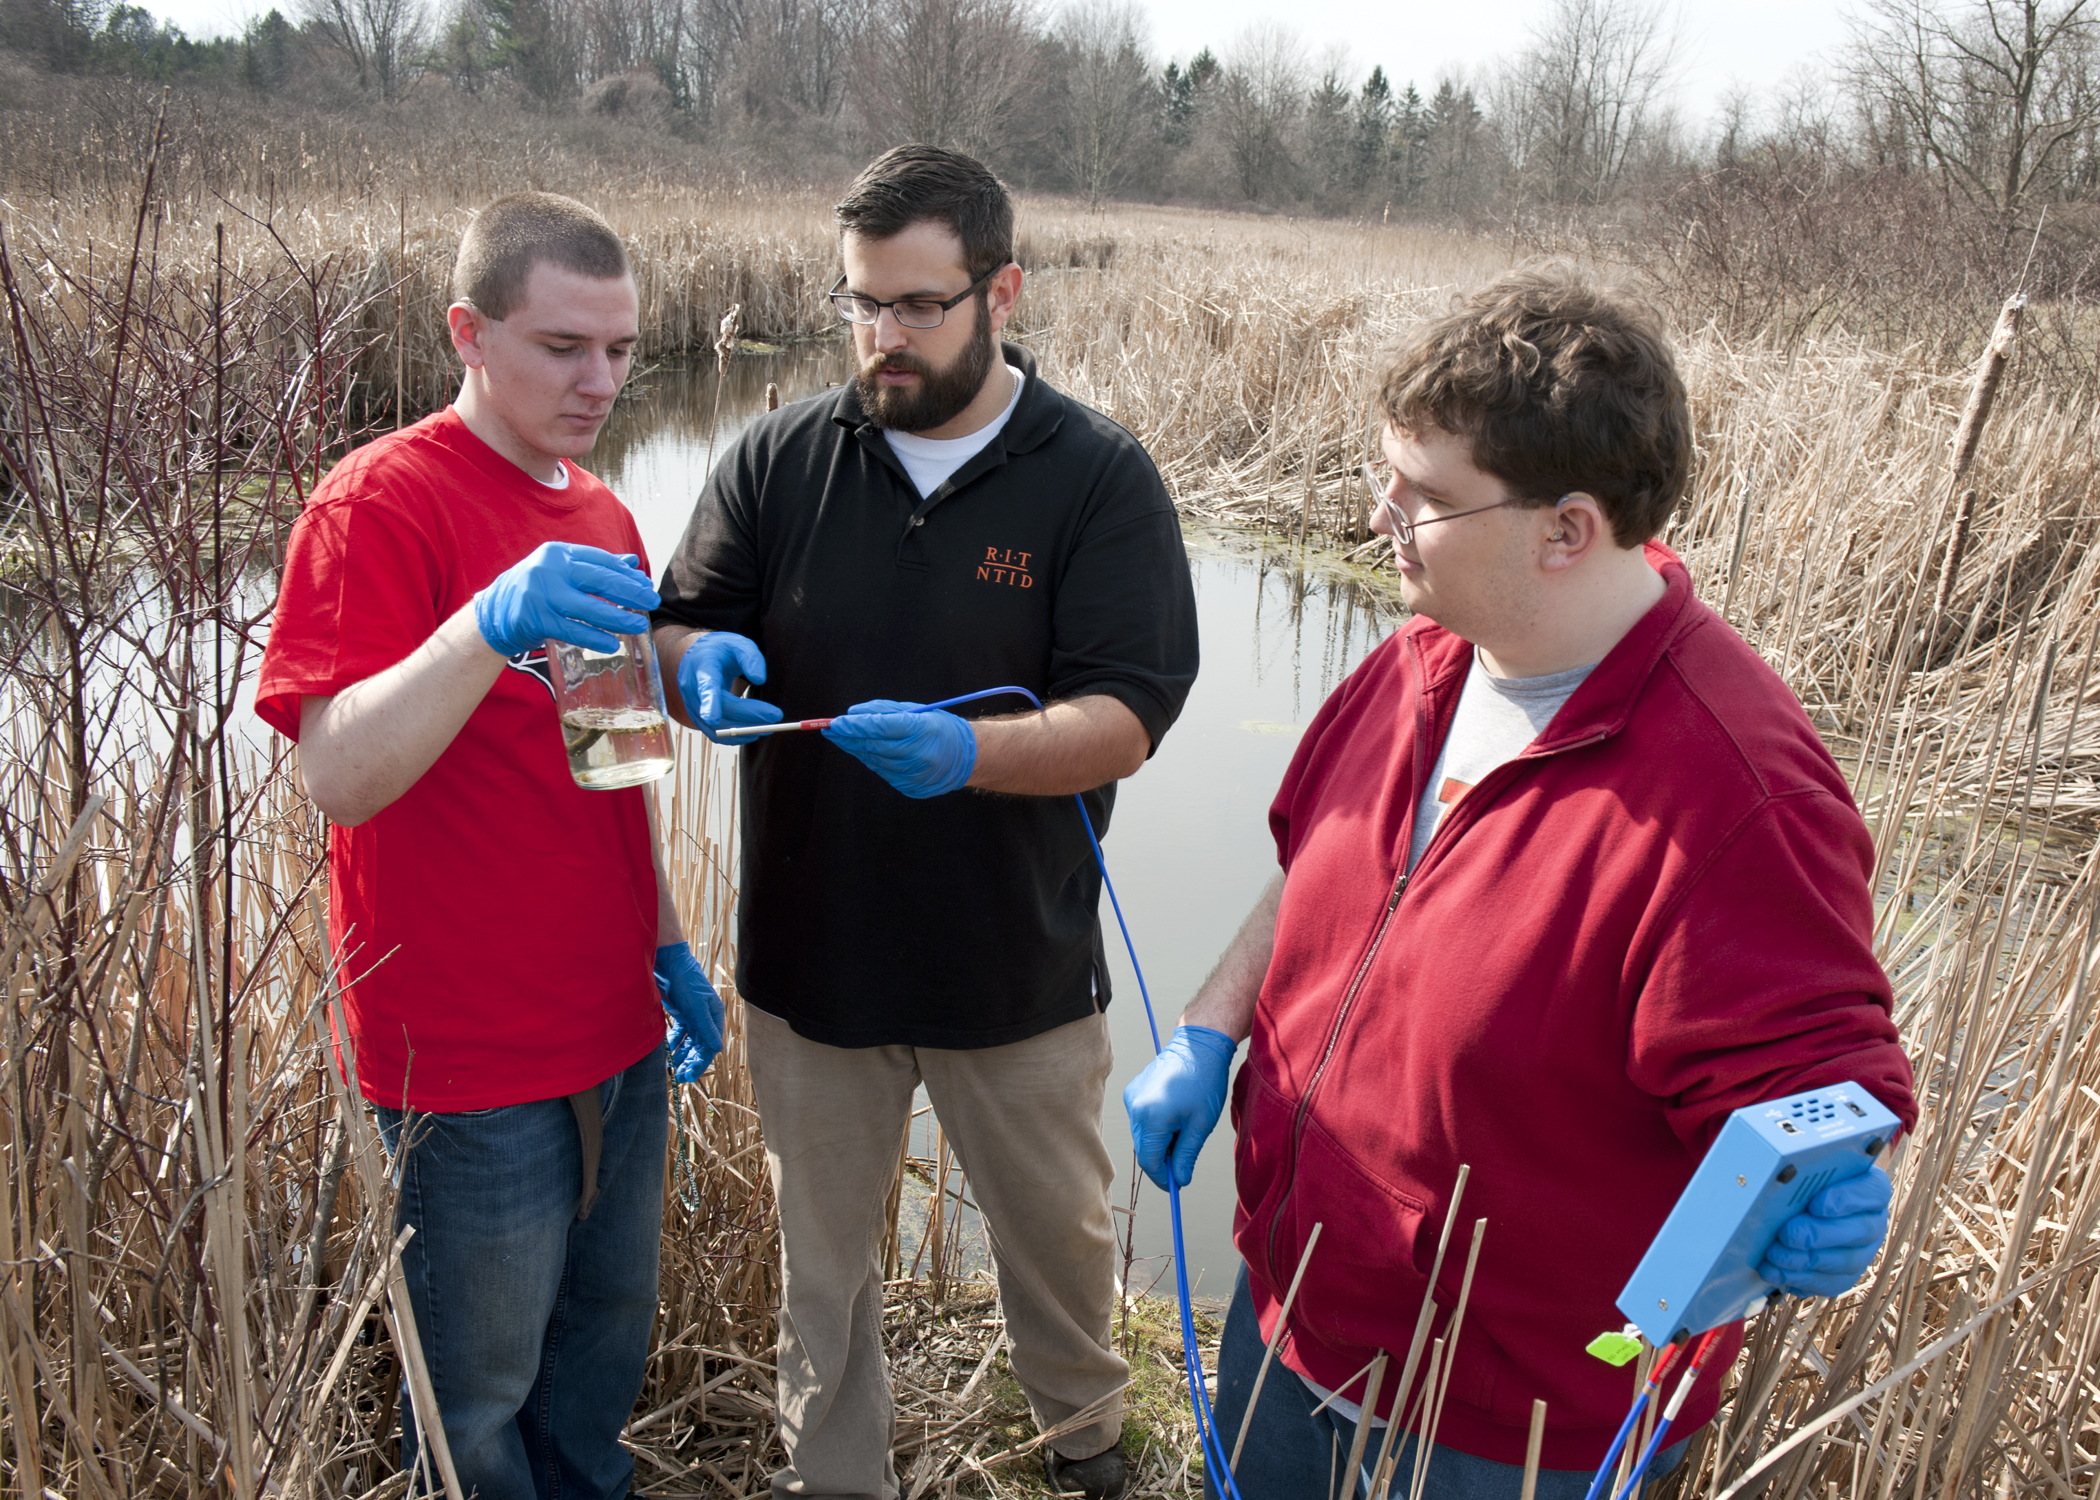
\includegraphics[width=1\linewidth]{Pagano_WaterTest.jpg}
\end{figure}

How did this mentee become a mentor (and related: how has transcendental literature made its way into this chemist’s integrated educational philosophy)? Yet again, it all comes back to Buckminster Fuller (my favorite interdisciplinary thinker and the protagonist of my teaching philosophy, published in \textit{JSESD} Vol. 16). I was introduced to his work by my doctoral advisor, Dr. Jonathan E. Kenny. He was perhaps my most substantial mentor, has become a friend, and remains one of my primary collaborators. Of course, I picked up most of my chemical research abilities under his tutelage, however, much of the teaching and professional successes that I have enjoyed can also be correlated to his mentoring. Coincidentally, we would often visit nearby Walden Pond to ponder science, life, teaching, and of course, the lives and times of Walden’s own Emerson and Thoreau. We would discuss how the two famous thinkers were known to interact with other local transcendentalists of their time, including Margaret Fuller- who coincidentally, is Buckminster Fuller’s great aunt. Margaret Fuller is credited with saying that “If you have knowledge, let others light their candles at it”. My mentor passed a ‘flame’ of invaluable knowledge to me. As a mentor, my mentor was a provider of the “flame”.

Certainly mentoring is not as easy as lighting one candle off another, with the ‘knowledge flame’ never really extinguishing as it is perpetually passed from mentor to mentee. However, a mentor can provide the tools and necessary encouragement for mentees to become self-confident and competent sources of strength unto themselves. Through support and encouragement from my mentors, I gained the courage, that when approached by senior faculty members early in my career telling me that my “wide-eyed passion for teaching was unsustainable”, I had the confidence to tell them (well, politely, of course) to get out of my path toward effective teaching and student success because I know it can be done (and I have seen it modeled by my own mentors). Today the roles are reversed and it is my turn to encourage a former student/ mentee (who is now a colleague) to stand up for herself as others might doubt her ability as a former deaf student to become a tenured professor and leader in academia. I am proud that she has risen to the occasion and is well on her way as a successful early-career professor. As a mentor, I am a provider of support and encouragement.

One of the most satisfying aspects of mentoring (and the whole of education, for that matter) is how it can be inherently cyclic in nature. I was mentored, and in turn, became a mentor to hundreds of D/HH individuals. Undoubtedly, and as it should be in the grand scheme of things, some of my mentees will become valued mentors to someone else- and so on into the future. I learn a great deal from my students and mentees. They have overcome deafness- some of them have secondary disabilities (low vision, mobility, etc.), and many of them are additionally from underrepresented/minority cultural groups. They are shattering the glass ceiling daily. And from them I have learned a great deal about perseverance, pride, and the profound societal advantages of diversity. I apply these lessons to the fabric my own life, and therefore, my mentees are my mentors. As a mentor, I am a provider of a seeming paradox (a cyclic source of mentoring unto myself).

\section*{BIOGRAPHICAL STATEMENT}

Dr. Todd Pagano is an Associate Professor of Chemistry at Rochester Institute of Technology and Director of the National Technical Institute for the Deaf’s Laboratory Science Technology program; a one-of-kind program in the world (i.e., a postsecondary chemical technology program for deaf and hard-of-hearing students). During his career at RIT/NTID, he has led the design and implementation of the LST program, set-up a state-of-the-art instrumentation laboratory, architected the new degree program, and helped to place a large number of deaf and hard-of-hearing individuals into careers in the chemical sciences. He received RIT’s Faculty Mentoring Award, is a Fellow of the American Chemical Society (ACS), and received the Dreyfus Foundation/ACS National Award: Encouraging Disadvantaged Students into the Chemical Sciences. He was named to the Rochester Business Journal’s “Forty Under 40” list and was also named a United States Professor of the Year by the Council for Advancement and Support of Education (CASE) and the Carnegie Foundation for the Advancement of Teaching

\end{large}
\end{document}
